\documentclass{article}
\usepackage{tempora}
\usepackage{indentfirst}
\usepackage{tabularx}
\usepackage{caption}
\usepackage{graphicx}
\usepackage{longtable}
\usepackage{tabularx}
\usepackage{amsmath}
\usepackage{amsfonts}
\usepackage{floatrow}
\floatsetup[table]{capposition=top}
\makeatletter
\graphicspath{ {./images/} }
\renewcommand*\l@section{\@dottedtocline{1}{1.5em}{2.3em}}
\makeatother
\usepackage{float}
\usepackage[english, russian]{babel}
\begin{document}
  \textbf{Постановка задачи}.

  Решается задача поиска оптимального распределения функционала программного средства по плагинам для интеграции в плагинную систему с уменьшенем связности его компонентов. При этом существуют ограничения на общее число используемых плагинов и на распределение функционала по ним. Функционал описан в требованиях к программному средству и реализован в файлах исходного кода на языке программирования.

  \begin{figure}[H]
      \centering
      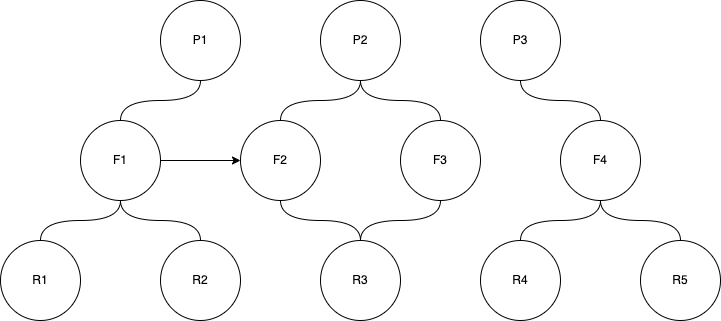
\includegraphics[width=1\textwidth]{Исходный граф.drawio}
      \caption{Граф $G$}
  \end{figure}

  Описание модели:
  \begin{itemize}
    \item требования $R$ в количестве $n$ штук.
    \item файлы исходного кода $F$ в количестве $m$ штук
    \item плагины $P$ в количестве $k$ штук
    \item требования трассируются на файлы исходного кода. Трассировка описана в матрице $E^{rf} = m \times n$
    \item файлы исходного кода имеют друг на друга зависимости. Сведения о зависимостях описаны в матрице $E^{ff} = m \times m$
    \item файлы исходного кода распределены по плагинам. Распределение описано в матрице $E^{fp} = k \times m$
    \item для упращения в задаче не учитывается ограничение на отсутствие циклических зависимостей между плагинами
  \end{itemize}

  Для описания включаемых и невключаемых в поставку требований, файлов и плагинов в задаче используются вектора значений. Активным называется элемент вектора, значение которого принимает положительное значение. Неактивным называется элемент вектора, значение которого равно $0$.

  Введем следующие обозначения:
  \begin{itemize}
    \item $R_{u}$ (useful requirements) - вектор требований. Активными элементами являются полезные требования в рамках поставки. Они подаются на вход модели. Значение активных элементов равно $1$
    \item $F^{t}_{u}$ (traceable useful files) - вектор файлов исходного кода. Активными являются те элементы, которые имеют трассируемость на активные элементы из $R_{u}$
    \item $F^{dep}_{u}$ (dependency useful files) - вектор файлов исходного кода. Активными являются те элементы, которые активны в $F^{t}_{u}$ и те, что необходимы для разрешения зависимостей активных в $F^{t}_{u}$ элементов
    \item $P^{t}_{d}$ (traceable delivery plugins) - вектор плагинов. Активными являются те элементы, которые содержат по меньшей мере один файл из $F^{dep}_{u}$
    \item $P_{d}$ (delivery plugins) - вектор плагинов. Активными являются те же элементы, что и в $P^{t}_{d}$. Значения активных элементов этого вектора равны $1$
    \item $F^{t}_{d}$ (traceable delivery files) - вектор файлов исходного кода. Активными являются те элементы, которые распределены по активным элементам из $P_{d}$
    \item $F_{d}$ (delivery files) - вектор файлов исходного кода. Активными являются те же элементы, что и в $F^{t}_{d}$. Значения активных элементов этого вектора равны $1$
    \item $R^{t}_{d}$ (traceable delivery requirements) - вектор требований. Активными являются те элементы, которые имеют трассируемость на активные элементы из $F_{d}$
    \item $R_{d}$ (delivery requirements) - вектор требований. Активными являются те элементы, которые активны в $R^{t}_{d}$ и имеют значение $1$
  \end{itemize}

  Поставка формируется для обязательного включения в нее всего полезного для заказчика функционала. Так же в нее включается бесполезный для заказчика функционал. Включение его необходимо для разрешения функциональных зависимостей. Отношение числа бесполезных требований к общему числу реализованных в поставке требований называется коэффициентом бесполезности: 
  \begin{center}
    $K_{un} = (\sum R_{d} - \sum R_{u}) / \sum R_{d}$ 
  \end{center}
  
  Для определения $R_{d}$ необходимо:
  \begin{enumerate}
    \item подать на вход модели $R_{u}$:

    \begin{center}
      $R_{u} = \{R_{1} = 1, R_{2} = 0, ..., R_{n} = 1\}$
    \end{center}

    \item рассчитать $F^{t}_{u}$:

    \begin{center}
      $F^{t}_{u} = R_{u} \cdot E^{rf}$
    \end{center}

    \item рассчитать $F^{dep}_{u}$. Достигается это путем сбора зависимостей у файлов на всей глубине вложенности зависимостей. Длина такой цепочки не может превышать общее число файлов. Поэтому достаточная глубина поиска зависимых файлов равна $m$. Для разрешения зависимостей можно использовать рекурсивную функцию:
    
    \begin{center}
    $
    D_{F}(x) = 
      \begin{cases}
        E^{ff} \cdot F_{n} & \quad \text{если } x = 1 \\
        E^{ff} \cdot D_{F}(x - 1) & \quad \text{если } x > 1
      \end{cases}
    $
    \end{center}

    Тогда:

    \begin{center}
      $F^{dep}_{u} = \displaystyle\sum^m_{i = 1}D_{F}(i)$
    \end{center}

    \item рассчитать $F_n$. Достигается это путем применения функции активации $A_{F}(x)$ к элементам $F^{dep}_{u}$:

    \begin{center}
      $
      A_{F}(x) = 
        \begin{cases}
          0 & \quad \text{ если } x = 0 \\
          1 & \quad \text{ если } x > 0
        \end{cases}
      $
    \end{center}

    \item рассчитать $P^{t}_{d}$:

    \begin{center}
      $P^{t}_{d} = F_{n} \cdot E^{fp}$
    \end{center}

    \item рассчитать $P_{d}$. Достигается это путем применения функции активации $A_{P}(x)$ к элементам $P^{t}_{d}$:

    \begin{center}
      $
      A_{P}(x) =
        \begin{cases}
          0 & \quad \text{ если } x = 0 \\
          1 & \quad \text{ если } x > 0
        \end{cases}
      $
    \end{center}

    \item рассчитать $F^{t}_{d}$:

    \begin{center}
      $F^{t}_{d} = E^{fp} \cdot P_{d}$
    \end{center}

    \item рассчитать $F_{d}$. Достигается это путем применения функции активации $A_{F}(x)$ к элементам $F^{t}_{d}$

    \item рассчитать $R^{t}_{d}$:

    \begin{center}
      $R^{t}_{d} = E^{rf} \cdot F_{d}$
    \end{center}

    \item рассчитать $R_{d}$. Достигается это путем применения функции активации $A_{R}(x)$ к элементам $R^{t}_{d}$

    \begin{center}
      $
      A_{R}(x) =
        \begin{cases}
          0 & \quad \text{ если } x < 1 \\
          1 & \quad \text{ если } x = 1
        \end{cases}
      $
    \end{center}

  \end{enumerate}

  Кроме того, существуют ограничения на значения элементов матриц $E^{rf}$ и $E^{fp}$.

  Ограничения на значения элементов матрицы $E^{rf}$:
  \begin{itemize}
    \item[] $0 \leq E^{rf}_{i, j} \leq 1$
    \item[] $E^{rf}_{1, 1} + E^{rf}_{1, 2} + ... + E^{rf}_{1, n} = 1$
    \item[] $E^{rf}_{2, 1} + E^{rf}_{2, 2} + ... + E^{rf}_{2, n} = 1$
    \item[] ...
    \item[] $E^{rf}_{m, 1} + E^{rf}_{m, 2} + ... + E^{rf}_{m, n} = 1$
  \end{itemize}

  Ограничения на значения элементов матрицы $E^{fp}$:
  \begin{itemize}
    \item[] 
    $
    E^{fp}_{i, j} =
      \begin{cases}
      0 \\
      1
      \end{cases}
    $
    \item[] $E^{fp}_{1, 1} + E^{fp}_{1, 2} + ... + E^{fp}_{1, n} = 1$
    \item[] $E^{fp}_{2, 1} + E^{fp}_{2, 2} + ... + E^{fp}_{2, n} = 1$
    \item[] ...
    \item[] $E^{fp}_{m, 1} + E^{fp}_{m, 2} + ... + E^{fp}_{m, n} = 1$
  \end{itemize}

  
  Задача заключается в поиске такого распределения файлов по плагинам, т.е. подборке значений элементов матрицы $E^{fp}$ при заданных $n$, $m$, $k$, $E^{rf}$ и $E^{ff}$, чтобы полученные от различных $R_{u}$ статистические показатели значений $K_{un}$ были бы минимальными. Под статистическими показателями здесь понимаются: сумма, среднее значение, математическое ожидание и т.д.

\end{document}
